\documentclass[11pt,twocolumn,varwidth=true,a4paper,fleqn]{article}
\usepackage{fullpage}
\usepackage{url}
\usepackage[margin=1.1in]{geometry}
\usepackage{graphicx}
\usepackage{csvsimple}
\usepackage{varwidth}
\usepackage{array}
\usepackage{float}
\usepackage{amsmath}
\usepackage{pgfplotstable}
\usepackage{amsmath }
\usepackage[T1]{fontenc}

\usepackage{authblk}

\author[1]{Bernstein Ran}
\author[2]{Shafir Tal}
\author[3]{Tsachor Rachelle}
\author[4]{Studd Karen}
\author[1]{Schuster Assaf}
\affil[1]{Department of Computer Science, Technion I.I.T, Haifa, Israel}
\affil[2]{The Graduate School of Creative Arts Therapies, University of Haifa}
\affil[3]{School of Theatre \& Music, The University of Illinois at Chicago}
\affil[4]{School of Dance, George Mason University}



\begin{document}
\nocite{*}
\newcolumntype{M}{>{\begin{varwidth}{3cm}}l<{\end{varwidth}}}


\title{Laban Movement Analysis using Kinect}
\maketitle
\begin{quote}{``Man moves in order to satisfy a need.`` ---\textup{Rudolph Laban}}
\end{quote}
\begin{abstract}
\textbf{Laban Movement Analysis (LMA) is a method for describing, interpreting
and documenting all varieties of human movement. Analyzing movements using LMA is advantageous over kinematic 
description of the movement, as it captures also qualitative aspects in addition to the 
quantitative aspects of the movement. As such, it has many applications and its popularity is 
increasing in recent years as the preferred method for movement analysis. This
study will develop an automated method for recognizing Laban motor elements from markerless 
3D movement data captured by a Kinect camera. Adequacy of the automated method will be established 
by applying it to emotion recognition from movement, comparing the results generated by the automated 
process to those collected from human perception. It obtained a recall
and precision rate of over 60\%  averaged over the elements.}
\end{abstract}
\section{Introduction}
The aim of our work is to create a method for an automated identification of the Laban motor elements 
(might be reffered also as qualities) that characterize any movement sequence,
using the Kinect sensor. We have created our own dataset, and applied several
Machine Learning (ML) techniques on it, in several learning settings. We chose
to use ML (instead of rule based algorithms), so we would be able to use
all of the rich data that is provided by the Kinect, and not to focus on a
very subttle feature extraction that requiers domain expertise and
limits the features to what is known. Using ML gave us the oppertunity to
do reverse engineering of the learned models, and learn about our problem's
intrinsic charecteristics.
\subsection{Motivation for Automated LMA}
The applications for computerized identification of the motor elements that characterize each possible 
human movement are numerous. For example: the generation and control of specific expressive movements 
of avatars, virtual characters, or robots in Mixed Reality scenarios; detection of personality traits 
during a job interview; early detection, severity assessment or revealing of genetic tendency (phenotype) 
towards various illnesses such as Alzheimer, autism, Parkinson�s disease, or schizophrenia, based on 
analysis of the person�s motor behavior; monitoring influences over time and early detection of deviation 
from normal behavior in closed environments such as space travel, and more. Automated emotion recognition 
from movement is another important application, which may have a variety of uses such as online feedback 
to presenters to help them convey through their body language the emotional message they want to communicate 
(e.g., politicians and public speakers; actors training); or emotion recognition of people�s emotions 
during interactive games such as those played using the Xbox. 
\\\\Our work on LMA is motivated by the correlation between LMA and emotional movements and emotions as 
stated by Shafir --- an expert researcher in the emotional movement domain. For that reason we narrowed 
recognition to only 18 Laban qualities (as listed in table \ref{mixedSummary}) that Shafir found to be
predictive for emotions.
\subsection{Laban movement analysis}
LMA is a formal language for motion description 
invented by Rudolf Laban \cite{Laban} in the middle of the 20th 
century. LMA describes, interprets, and documents mental 
states from both conscious and unconscious human 
motion based on Laban's categories of body, effort, shape, 
and space. LMA has been used in the fields of dance, 
acting, athletics, physical therapy, and psychology and 
behavioral science. Laban exercises are based on the belief that by observing and analyzing 
movements, both conscious and unconscious, it is possible to recognize the objectives 
of the mover and to become aware of an inner attitude that precedes an action. Laban 
helps actors create momentary moods and long-standing personality traits 
through movement. For example, LMA work investigates the effort properties ---
flow, space, time and weight --- of all movement and helps actors think
specifically about why their character might move in a jerky, fast, light and direct manner
verses a heavy, slow, indirect and uninterrupted manner.
The effort properties are defined as follows:
\begin{itemize}
\item
Flow: Bound or Free 
\item
Space: Direct or Indirect 
\item
Time: Sudden or Sustained 
\item
Weight: Strong or Light 
\end{itemize}
\begin{figure*}[ht]
\centering
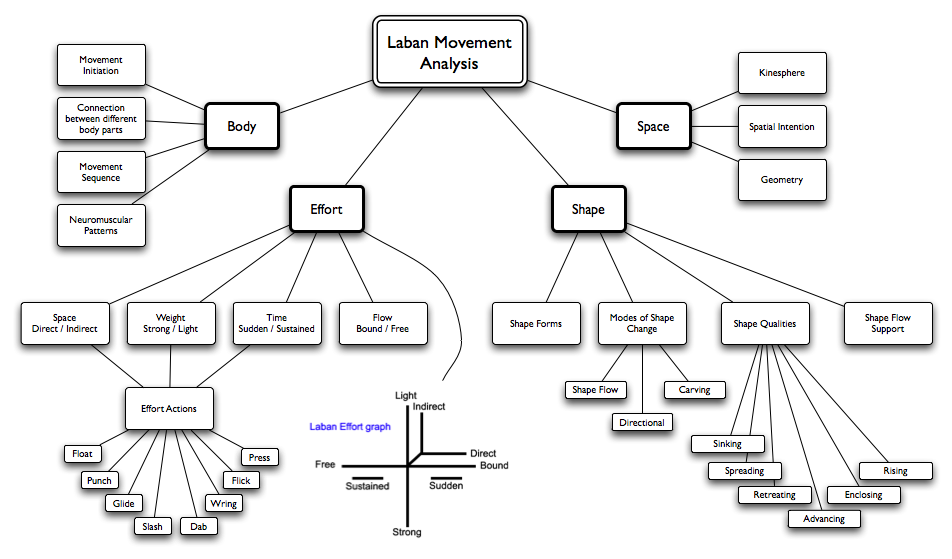
\includegraphics[width=\textwidth]{laban.png}
\caption{Main axes of LMA. Taken from \cite{labanTree}}
\label{labanTree}
\end{figure*}
The entire LMA hierarchy is showon in figure \ref{labanTree}.

\subsection{Kinect Sensor Data}
This following figure shows the skeleton provided by Kinect's
software development kit and used in this paper.
\begin{figure}[h]
\centering
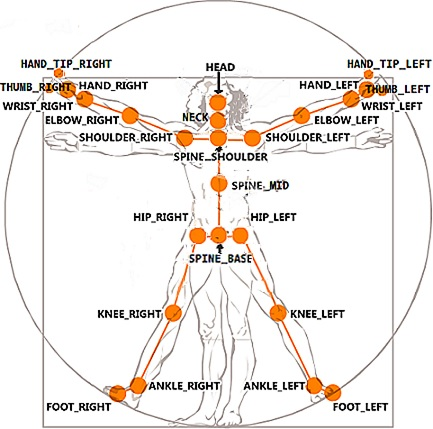
\includegraphics[width=60mm]{skeleton.jpg}
\caption{Skeleton positions relative to the human body}
\label{skeleton}
\end{figure}
Once the skeleton is detected, the 3D coordinates of all the joints of the
user's body --- with the exception of joints that are not visible (e.g. a user's
hand is behind his or her back) --- are provided.
As seen in Figure \ref{Coordinate}, the coordinates are in a ``real-world''
coordinate system, whose origin [0,0,0] is in the sensor and whose x-, y-, and
z-axis are as depicted below;
\begin{figure}[h]
\centering
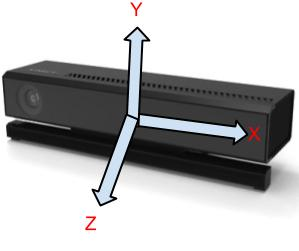
\includegraphics[width=60mm]{KinectV2CoordinateSystem.jpg}
\caption{Kinect Coordinate System}
\label{Coordinate}
\end{figure}

\subsection{Related Work}
Several attempts were made to recognize Laban qualities,
most of them for emotion recognition in the context of Human Robot Interaction (HRI).
Martin et al. \cite{martin} analyzed the importance of gestures in emotion
recognition for HRI. Masuda et al. generated emotional body motion for a human 
form robot \cite{Masuda}. Rett et al. proposed a human motion recognition 
system using a Bayesian reasoning framework \cite{Rett}. Gabel et al.
\cite{gabel2012full} used the Kinect sensor for gait analysis. The works of
Zacharatos et al. \cite{Zacharatos} and Kim et al. \cite{kim} were inspired by LMA
for emotion recognition using the Kinect sensor. The last two works based
their feature extraction method on LMA principles, but did not attempt try to
recognize the qualities themselves. In this paper we deal only with recognition of Laban
qualities.

\section{Method}
The due to the fact that we are the first to handle Laban recognition with
Kinect V2, we had to create a dataset from scratch. To reduce the noise, and for
being sure that we capture the essence of the Laban qualities in our dataset, we
decided that most of the dataset will come from recording CMAs, and the rest
will be recording of ordinary people. 
\subsection{Clip Collection}
Two main datasets were collected: 
\begin{itemize}
  	\item 
	Certified Movement Analyst (CMA) dataset - includes 6 CMAs performing in about
	80 clips each (a total of 550 clips). Every clip is 3 seconds long, and
	the CMA performs random activity in it. To achieve uniform distribution of the Laban
	qualities over the dataset, in every clip the CMA was asked to perform
	actions that include several specific qualities, and nothing but them.
	
	\begin{figure}[h]
	\centering
	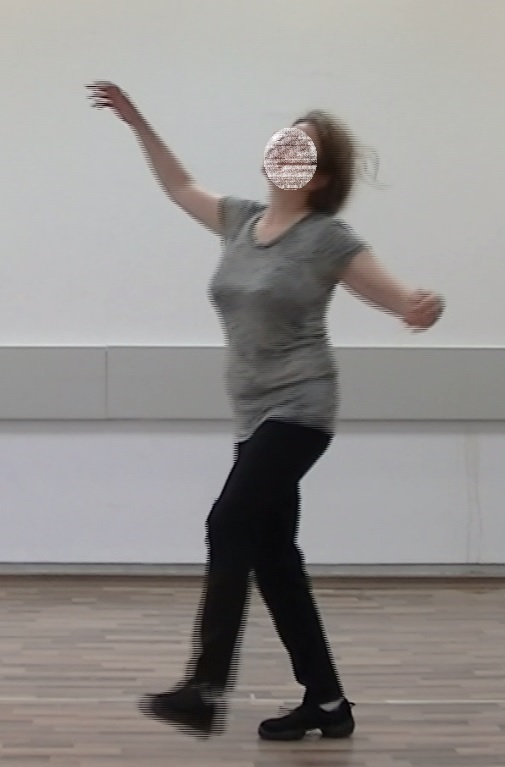
\includegraphics[width=30mm]{Rachelle.jpg}
	\caption{CMA during a clip}
	\label{Rachelle}
	\end{figure}
	
	\item 
	Non-CMAs dataset - includes 2 subjects without a background in movement
	analysis, performing 30 clips each. Every clip is also 3 seconds long,
	and the subject was asked to perform one out of several
	tasks.
\end{itemize}
\subsection{Clip Labeling}
To achieve a ground truth labeling for the two datasets, every clip was tagged by
a committee of 2 CMAs who determined which Laban qualities appear in the
clip. The use of a committee decision instead of the subjective opinion of one
CMA decreases the labeling noise and the decision is considered as ground truth.
We believe this is justifiable in light of the fact that there is no real
ground truth in such a nonquantitative method as LMA.
\subsection{Feature Extraction}
Due to the unequal length of clips, all the extracted features are in whole clip 
granularity.
\subsubsection{General Low Level Features}
For every joint in the skeleton, the angular velocity, acceleration, and jerk
were extracted, and for every pair of joint and metric, the mean, variance,
skew, and kurtosis were extracted (the extraction of the last four moments
is denoted as $\phi$).
\subsubsection{LMA Shape Analysis: Sagittal Plane}
The Laban's shape analysis of the sagittal plane is the distinction
between Advance and Retreat. This distinction was quantified by projecting the 
speed vector of the Center Of Mass (COM) on the vector of the front of the body. 
The COM was approximated in this case by the average of all of the joints. 
The front of the body was approximated by the perpendicular vector to the vector 
between the Left Shoulder (LS) and
the Right Shoulder (RS).
\\\\If $\vec{P}_{j}(t)$ is the vector of the position of joint j in time t in
a clip with n frames, and $ \alpha_{j}$ is a coefficient proportional to the
mass around of the joint:
\\
\\$\vec{P}_{COM}(t) = \sum_{j \in Joints} \alpha_{j}\vec{P}_{j}(t),
\\
\\\vec{P}_{shoulders}(t)=\vec{P}_{LS}(t)-\vec{P}_{RS}(t),$
\\
\\\[ \vec{P}_{front}=\vec{P}_{shoulders}\left( \begin{array}{ccc}
0 & 0 & 1 \\
0 & 1 & 0 \\
-1 & 0 & 0 \end{array} \right)\],
\\
\\
$S_{sag}(t) = \vec{P}_{COM}(t)\cdot\vec{P}_{front}(t),$
\\
\\
$\vec{F}_{sag} = \phi([S_{sag}(1), \ldots S_{sag}(n)]),$
\\\
where $\phi$ denotes extraction of the moments.
\subsubsection{LMA Shape Analysis: Horizontal Axis}
Here the distinction is between spreading and enclosing on the horizontal axis.
This distinction was quantified by measuring the average distance of the joint from 
the vertical axis of the body that spreads from the Head (H) to the Spine Base (SB).
\\
\\$d_{j} = \frac{\left|(\vec{P}_{j}-\vec{P}_{SB})\times
(\vec{P}_{j}-\vec{P}_{H})\right|}{\left|\vec{P}_{H}-\vec{P}_{SB}\right|},
\\
\\S_{horiz}(t) = \sum_{j \in Joints} d_{j}(t),
\\
\\\vec{F}_{horiz} = \phi([S_{sag}(1), \ldots S_{sag}(n)]),$
\\where $\phi$ denotes the extraction of the moments.
\subsubsection{LMA Shape Analysis: Vertical Axis}
Here the distinction is between rise and sink on the vertical axis.
This distinction was quantified by measuring the average distance on axis y of each
joint from the COM. This quantification is based on the assumption that the body
is ``longer'' when rising.
\\
\\$S_{vert}(t) = \sum_{j \in Joints}
\left|\vec{P}_{j}-\vec{P}_{COM}\right|,
\\
\\\vec{F}_{vert} = \phi([S_{sag}(1), \ldots S_{sag}(n)]),$
\\where $\phi$ denotes the extraction of the moments.
\subsubsection{LMA Effort Analysis: Time Category}
Here the distinction is between sudden or sustained. This quality was 
quantified by the skew of the acceleration, relying on the assumption that the
acceleration of a sudden movement will be skewed further to the left, i.e., will get
a higher value at the beginning of the movement.
\subsubsection{LMA Effort Analysis: Space Category}
Here the distinction is between direct and indirect motion. This quality was 
quantified by the angle between the movement vector of a joint to the next one,
relying on the assumption that in direct movement every vector will be in
the same direction as the last (the angle between them is small).
\\\\If $\vec{P}_{j}(t)$ is the vector of the position of joint j in time t, the
movement vectors are:
\\\\$\vec{V}_{j}(t) = \vec{P}_{j}(t+1) - \vec{P}_{j}(t).$
\\\\The angles between them are calculated with inner products:
\\\\$\vec{A}_{j}(t) = \vec{V}_{j}(t+1) \cdot \vec{V}_{j}(t).$

\subsection{Performance Evaluation}
There are 18 labels (Laban qualities) that can be assigned to every clip, but
a typical clip usually includes about 3 qualities, which means that there is
about 85\% chance that a quality won't appear in a clip. Due to
this sparsity, accuracy alone is not a relevant metric for the
performance evaluation because one can get the an 85\% accuracy by stating that
for every recording none of the qualities appear. A better evaluation would have to
combine the precision and recall rates of the classifier. This can be done using 
the F1 score:
\\
\\$F_{1} = \frac{2\cdot precision\cdot recall}{precision+recall}.$
\subsection{Feature Selection}
	Every clip is extracted into a vector of 6120 features. Most of
	them are noisy or redundant. For that reason massive feature selection is
	needed. The feature selection is done in three stages:
	\begin{itemize}
		\item
		Computing the Anova F-value for every feature over the training set. Cross 
		validation was used to determine the optimal number of features that should be
		left. As it seen in Figure  \ref{selection}, the result was that the filtering
		out most of the features yielded better results than not filtering them, where
		using the top 4\% of features was optimal.
		\begin{figure}[ht!]
			\centering
			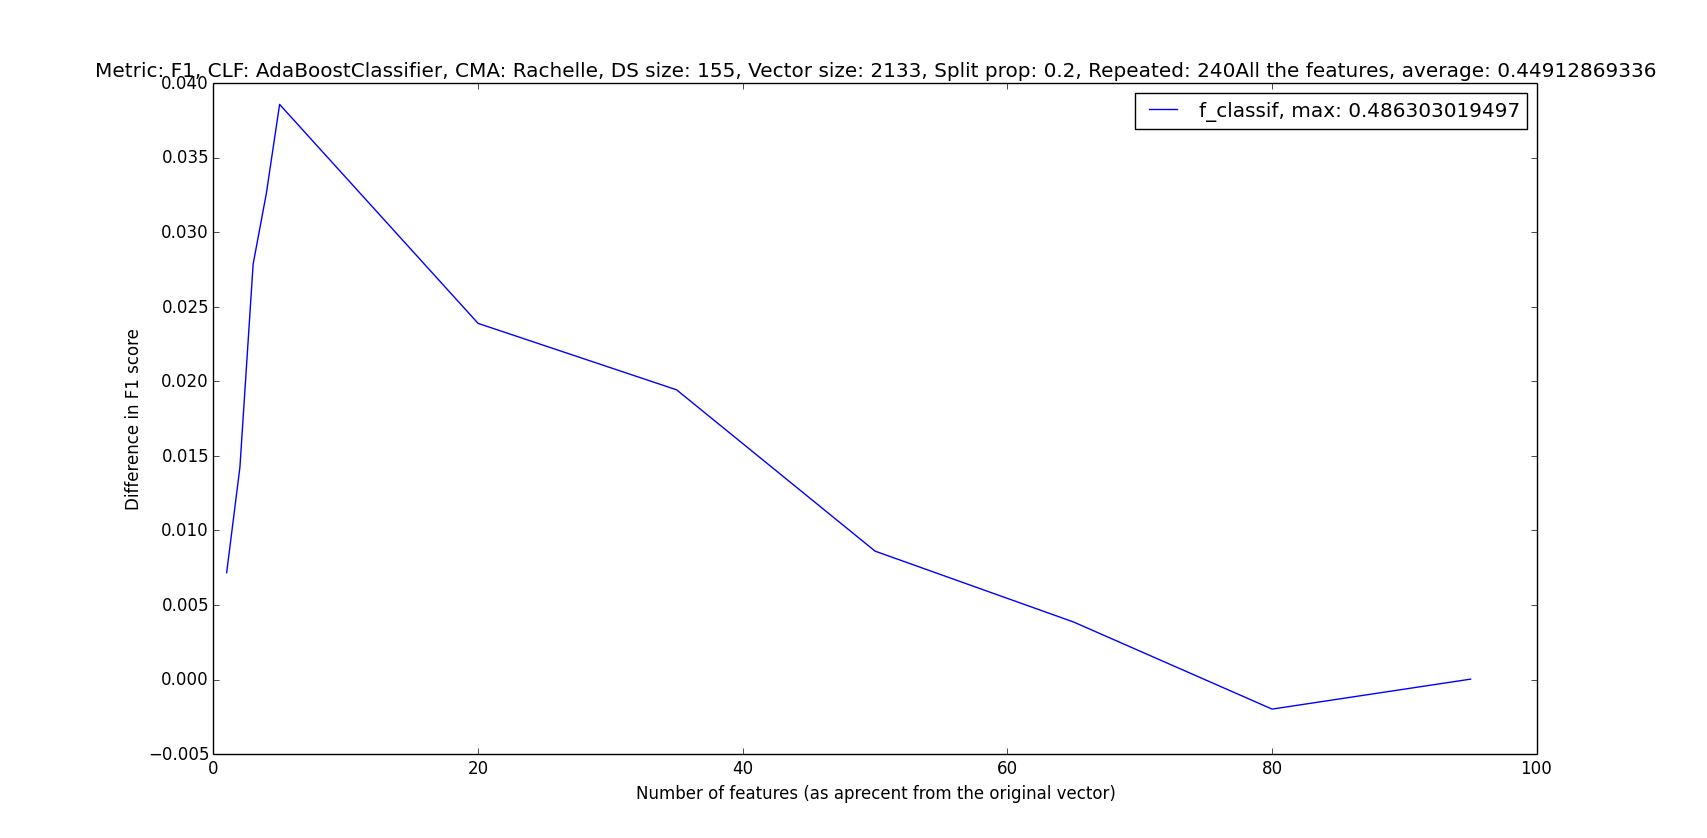
\includegraphics[width=70mm]{featureSelection.png}
			\caption{Influence of the amount of features on the performance. The
			selection was made according to statistical significance.
			The blue line is the difference between the score with and without feature
			selection. It can be seen that the optimal fraction of features to select is
			4\%.}
			\label{selection}
			\end{figure}
		\item
			The second phase of feature selection was conducted by Information Gain (IG)
			rating of the features. As it seen in figure  \ref{igFromFclassif}, the optimal ratio
			was selecting the top 60\% out of the features that have survivied the first
			phase of feature selection.
			 \begin{figure}[h]
				\centering
				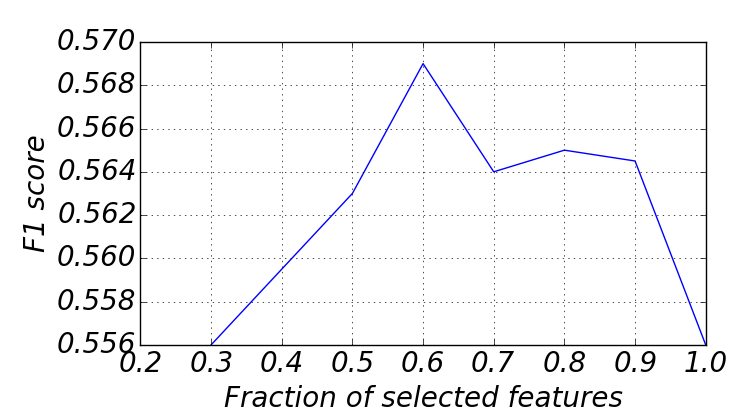
\includegraphics[width=70mm]{igFromFclassif.png}
				\caption{Influence of the amount of features selected with IG from the subset
				of features that was chosen in the first phase on the performance. The
				optimal ratio was 60\%.}
				\label{igFromFclassif}
			\end{figure}
			Examples of qualities and their most significant feature are given in 
			table \ref{bestFeatures}. The ``Information Gain'' metric used
			in the table is defined as:
			\begin{equation*}
			       IG(T,f) = H(T) - H(T|f),
			\end{equation*} 
			where T is the training set, f is a feature, and H() is the information
			entropy of a dataset.
			 \begin{table*}[ht!]
			   \centering
			   \csvautotabular{rankFeatures.csv}
			   \caption{Example of several qualities and the feature found to be
			   the most informative for them. ``Relative position'' stands for the
			   position of the joint relative to the ancestor joint in the joint
			   hierarchy.}
			   \label{bestFeatures}
			\end{table*}
		\item
		The third phase of feature section was conducted using the Least Absolute Shrinkage and
		Selection Operator (LASSO) regularization.
	\end{itemize}

\section{Experimental Setups and Results}
\subsection{Multilabel Classification}
Multilabel learning deals with the problem where each instance is associated
with multiple labels simultaneously, where the number of labels is not fixed
from instance to instance. The task of this learning paradigm is to predict
the label (Laban quality) set for each unseen instance (skeletal recording), 
by analyzing training instances with known label sets. The multilabel
approach taken in this paper is to break the whole LMA problem into 18
binary classification tasks --- one for every Laban quality - where every binary
decision is whether or not the quality exists.
\\The following subsections will describe several experimental setups
where the results in each will serve as a baseline for the next.
\subsection{Per CMA Evaluation}
	In this experiment the train and test datasets are taken from the same
	CMA. The average performance over the different CMAs is shown in Table
	\ref{oneCMASummary}. The performance on every Laban quality separately
	is demonstrated on a dataset of one of the CMAs in figure \ref{oneCMAFinal}.
	In tables \ref{oneCMAFinal} and \ref{mixedCMASummary} the incremental evolution
	of the algorithm is described from step to step with the next notation:
	\begin{itemize}
	\item 
	\textit{Chance} stands for randomly tossing a balanced coin in every
	classification decision.
	\item 
	\textit{Nearest Neighbors} stands for applying the Nearest Neighbors algorithm.
	\item 
	\textit{LinearSVC} stands for Support Vector Classifier with a linear
	kernel.
	\item 
	\textit{Label Balancing} stands for giving greater weight to clips that
	contain the quality due to the small fraction of them in the whole
	dataset.
	\item 
	\textit{Lasso}, \textit{Statistical Feature Selection}, and \textit{IG Feature
	Selection} were described in the feature selection section.
	\end{itemize}
	 \begin{table}[H]
	  	\centering
		\begin{tabular}{|p{1.6cm}|p{0.9cm}|p{0.9cm}|p{0.9cm}|p{0.9cm}|}
		\hline
		Algorithm /Metric&Preci-sion&Recall&F1&F1 SD\\\hline
		Chance&0.15&0.50&0.23&0.01\\\hline
		Nearest Neighbors&0.30&0.24&0.26&0.05\\\hline
		LinearSVC &0.35&0.39&0.37&0.04\\\hline
		Label Balancing&0.39&0.42&0.41&0.05\\\hline
		Lasso&0.41&0.48&0.44&0.05\\\hline
		Statistical Feature Selection&0.44&0.51&0.48&0.09\\\hline
		IG Feature Selection&0.48&0.59&0.53&0.09\\\hline
		\end{tabular}
		\caption{Evaluation every CMA's dataset separately in single task learning
		setting. Each row represents an additional step in the algorithm's evolution.
		The results are the average performance and standard deviation (SD) over the CMAs.}
	   \label{oneCMASummary}
	\end{table}

	\begin{figure*}[ht!]
		\centering
		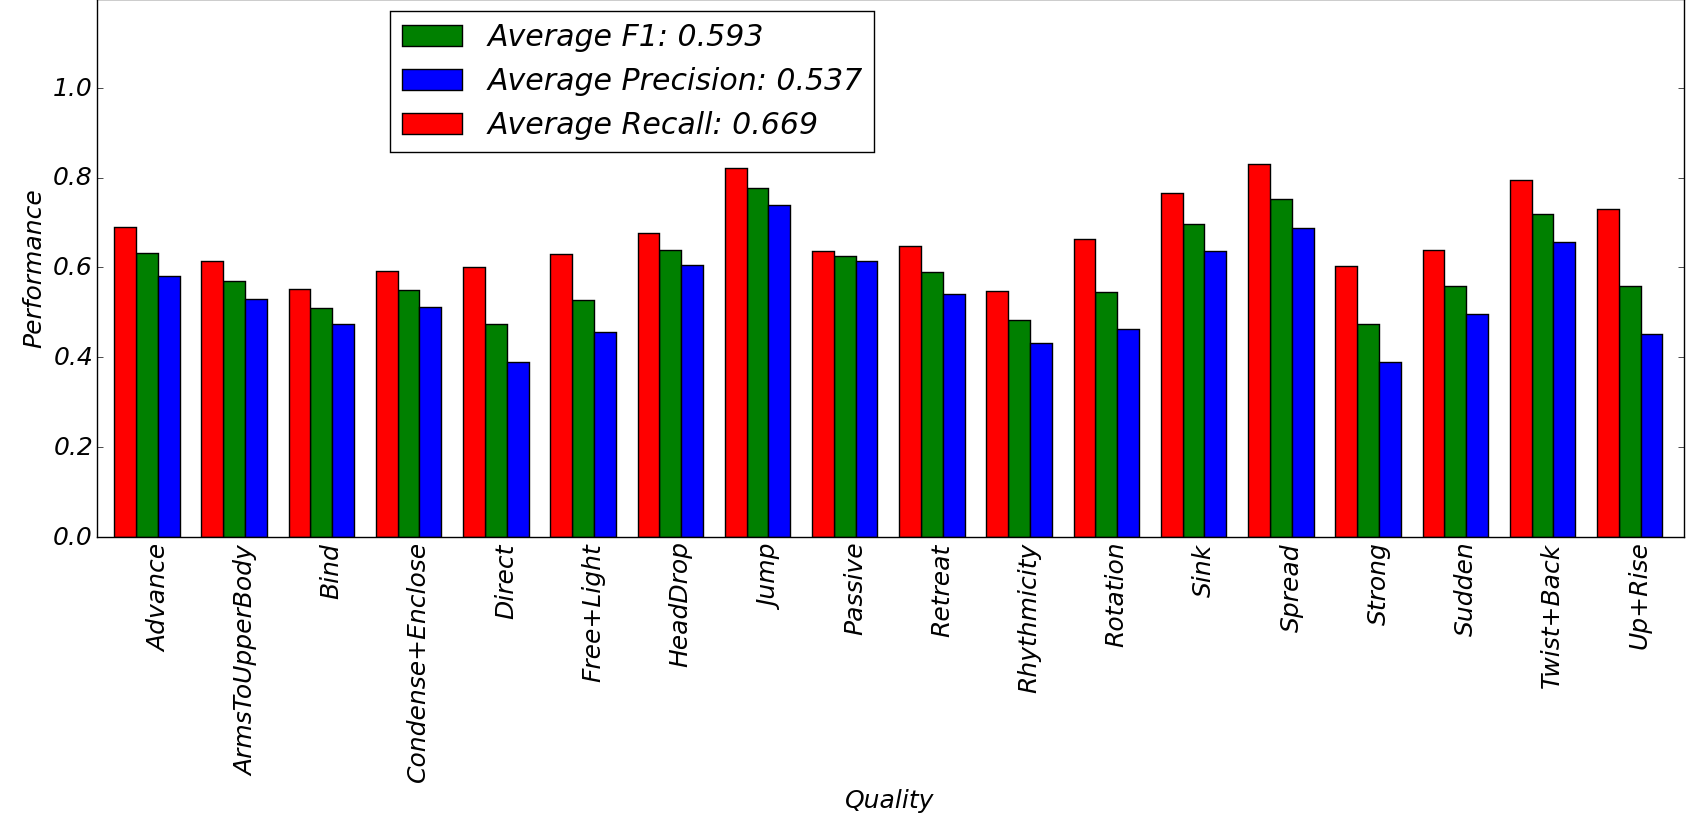
\includegraphics[width=\textwidth, height=60mm]{oneCMAFinalWithoutTitle.png}
		\caption{Recall, precision and F1 score of each Laban quality separately. The
		evaluation was conducted on a dataset that was captured on only one CMA. 
		Averaged over the qualities scores of the qualities are shown in the legend.}
		\label{oneCMAFinal}
	\end{figure*}
	
\subsection{Mixed Dataset Evaluation}
	In this section the datasets of all of the CMAs were mixed. In the learning
	and testing process the origin (CMA) of the sample was ignored. 
\subsubsection{Single Task Learning as a Baseline}
As a baseline we applied the SVM based flow that was described in the last
section on the mixed dataset. The results are shown in Table
\ref{mixedCMASummary}.
\begin{table}[ht!]
	  	\centering
		\begin{tabular}{|p{1.6cm}|p{0.9cm}|p{0.9cm}|p{0.9cm}|p{0.9cm}|}
		\hline
		Algorithm /Metric&Preci-sion&Recall&F1\\\hline
		Chance&0.15&0.50&0.23\\\hline
		Nearest Neighbors&0.41&0.235&0.3\\\hline
		LinearSVC &0.4&0.43&0.418\\\hline
		Label Balancing&0.394&0.47&0.43\\\hline
		Lasso&0.4&0.45&0.42\\\hline
		Statistic Feature Selection&0.462&0.69&0.55\\\hline
		IG Feature Selection&0.46&0.71&0.56\\\hline
		\end{tabular}
		\caption{Evaluation on CMA mixture dataset in single task learning
		setting. Every row is an additional step in the algorithm's evolution.}
	   \label{mixedCMASummary}
	\end{table}
It can be seen that there an improvement of the performance in a compare to the
per CMA evaluation of the last section. We explain the improvement with two
reasons -- the growths of the dataset's size when merging few CMAs'
datasets together, and the diversity of the clips which helps the model's
generalization.
\subsubsection{Multitask vs Single Task Learning}
We found that multitask learning for all the 18 qualities together exhibited superior 
performance to learning a classifier for each problem separately. For the
multitask instance we used Multitask Elastic Net (MEN) regularization, which is
the multitask regularization method of Zou et al. \cite{Zou}, where the
optimization objective is:
\\
\begin{equation}\label{eq:MEN}
	\|Y - XW\|^2_F+\lambda_1\cdot\|W\|_{2,1}+\lambda_1\cdot\|W\|^2_F,
\end{equation}    
  
$\lambda_1$, and $\lambda_2$ are hyper parameters, where,
\\
\begin{equation*}
        \|W\|_{2,1} = \sum_i \sqrt{\sum_j w_{ij}^2},
\end{equation*} 
    i.e., the sum of norm of each row (also known as mixed norm), and 
\begin{equation*}
        \|W\|^2_F = \sum_i{\sum_j w_{ij}^2},
\end{equation*}     
	i.e., the Frobenius norm. 

Feature selection was carried out by averaging the statistical significance of
each feature with respect to different tasks (This is in contrast to the single
task learning flow, where every task had its own feature selection). As seen in
Table \ref{MultitaskVsSeparated} the multitask setting improved the F score by
7\%, indicating that the tasks are correlated and more might be learned
from the small dataset when using this setting.	
 	\begin{table}[H]
	  	\centering
		\begin{tabular}{|p{1.8cm}|p{1.8cm}|p{1.8cm}|}
		\hline
		Metric&Single task&Multitask\\\hline
		Precision&0.46&\textbf{0.59}\\\hline
		Recall&\textbf{0.71}&0.65\\\hline
		F1&0.56&\textbf{0.6}\\\hline
		\end{tabular}
		\caption{Multitask vs Single task learning performance evaluation on mixture
		of CMAs dataset.}
	   \label{MultitaskVsSeparated}
	\end{table}

\subsubsection{Performance of Every Quality in Multitask Setting}
The performance over every quality as classified by the MEN in Table
\ref{mixedSummary}. During the MEN optimization ~\eqref{eq:MEN}, the mixed norm 
term $\|W\|_{2,1}$  promotes sparsity in the weights matrix $W$ such that for 
every row in the matrix, if one coordinate is equal to zero, then every coordinate 
in the row will be equal to zero.
\\The generalization ability of the model was enhanced by the fact that the
decision which features to select is influenced by all the qualities, (feature $f_i$ is selected in the MEN if the row $r_i$ in $W$ is not all 
zero), especially those that performed worse in the single task learning
setting (strong, and sudden for example).
\begin{table}[ht!]
	  	\centering
		\begin{tabular}{|p{3cm}|p{0.9cm}|p{0.9cm}|p{0.9cm}|}
		\hline
		Quality&Precis-ion&Recall&F1 score\\\hline
		Jump&0.89&0.81&0.85\\\hline
		Twist+Back&0.69&0.85&0.76\\\hline
		Sink&0.62&0.79&0.69\\\hline
		Rhythmicity&0.59&0.72&0.65\\\hline
		Spread&0.55&0.76&0.64\\\hline
		Head drop&0.60&0.66&0.63\\\hline
		Rotation&0.66&0.60&0.63\\\hline
		Free and Light&0.45&0.94&0.61\\\hline
		Up and Rise&0.67&0.54&0.60\\\hline
		Condense and Enclose&0.44&0.84&0.58\\\hline
		Arms To Upper Body&0.67&0.54&0.60\\\hline
		Advance&1.00&0.38&0.55\\\hline
		Retreat&0.50&0.59&0.54\\\hline
		Passive&0.40&0.85&0.54\\\hline
		Bind&0.44&0.61&0.51\\\hline
		Direct&0.56&0.49&0.52\\\hline
		Sudden&0.61&0.41&0.49\\\hline
		Strong&0.29&0.42&0.34\\\hline
		\textbf{Average}&\textbf{0.59}&\textbf{0.65}&\textbf{0.60}\\\hline
		\textbf{SD}&\textbf{0.17}&\textbf{0.17}&\textbf{0.11}\\\hline
		\end{tabular}
		\caption{Recall, precision and F1 score of each Laban quality on a CMA
		   mixture dataset. The learning was done in a multitask setting. The number of
		   features that weren't nullified by the mixed norm regularization is
		   282 (same features for all of the tasks). The F1 average and standard
		   deviation over the qualities is shown in the last row of the table.}
	   \label{mixedSummary}
	\end{table}

\subsection{Evaluation on a New CMA}
In this experiment the test set was taken from a CMA who did not appear in
the train set. As shown in Table \ref{domainAdaptationBaseLine}, 
performance degrades on the new CMA.

\begin{table}[H]
  	\centering
	\begin{tabular}{|p{3.5cm}|p{0.9cm}|p{0.9cm}|p{0.7cm}|}
	\hline
	Metric&Precis-ion&Recall&F1\\\hline 
	Average Score&0.57&0.58&\textbf{0.57}\\\hline
	Standard deviation between qualities&0.12&0.08&0.08\\\hline
	Average (over qualities) standard deviation within a
	quality&0.17&0.25&0.15\\\hline
	Standard deviation between CMAs&0.03&0.09&0.06\\\hline
	Average (over CMAs) standard deviation within a CMA&0.2&0.23&0.16\\\hline
	\end{tabular}
	\caption{Quality detection performance on a new subject. In every
	trial one CMA was the test set, while the classifier was learned from the
rest.}
   \label{domainAdaptationBaseLine}
\end{table}

We blame the degradation on the large variability between clips from
one CMA to another. Every CMA performed different gestures, in different
postures (some sitting and some standing) and in different contexts (some were
dancing while some where acting).

\subsection{Validation on Ordinary People}
The final validation was conducted on ordinary people (non CMAs). We
designed several daily actions (greeting friends or playing with a balloon, for
example) and the CMA committee tagged the clips. This dataset was small with a
focus on the elements shown in table \ref{nonCMAs}.

\begin{table}[H]
\centering
\begin{tabular}{|p{3cm}|p{0.9cm}|p{0.9cm}|p{0.9cm}|}
	\hline
	Quality&Precis-ion&Recall&F1 score\\\hline
	Jump&0.69&0.75&0.72\\\hline
	Spread&0.53&0.82&0.65\\\hline
	Arms to Upper Body&0.5&0.5&0.5\\\hline
	Free and Light&0.53&0.48&0.5\\\hline
	Sink&0.45&0.58&0.5\\\hline
	Condense and Enclose&0.4&0.5&0.45\\\hline
	Rotation&0.3&0.86&0.45\\\hline
	\end{tabular}
	\caption{Performance on ordinary people (non-CMAs) instructed to
	   perform several tasks.}
\label{nonCMAs}
\end{table}

\section{Conclusion}
Our method obtained a recall and precision of over 60\% over the qualities. 
There are a few Laban qualities, such as strong, that we found more 
difficult to quantify in bio-mechanical measurements. Overall we believe
that we succeeded capturing the essence of most of the qualities with a
100\$ sensor, which will make the LMA method applicable in many more
methodologies and processes.
\bibliographystyle{unsrt}
\bibliography{bib}

\end{document}
